\documentclass{article}
\usepackage[UTF8]{ctex}
\usepackage[tc]{titlepic}
\usepackage{amsmath, amsthm, amssymb, graphicx}
\usepackage{hyperref}
\usepackage{listings}
\usepackage{titlesec}
\usepackage{cite}
\usepackage{fancyhdr}
\usepackage{booktabs}
\usepackage{graphicx}
\usepackage{geometry}
\usepackage{caption}
\usepackage{subfigure}
\usepackage[section]{placeins}
\geometry{a4paper,scale=0.8}
\pagestyle{fancy}

\lhead{第 2 次作业\\\today}
\chead{中国科学技术大学\\数学建模课程}

\rhead{Assignment 1\\ {\CTEXoptions[today=old]\today}}
\newcommand{\upcite}[1]{\textsuperscript{\cite{#1}}}

\titleformat*{\section}{\bfseries\Large}
\titleformat*{\subsection}{\bfseries\large}

\title{\bfseries 基于SVD与RSVD方法的图像压缩}
\author{Xiaoma \quad   \quad  }

\begin{document}
\maketitle
\begin{abstract}
    在现实世界中,我们经常需要对图像进行传输或存储,图像的大小与传输和存储的成本
    密切相关,所以我们需要在尽可能保证图像质量的前提下,采用相应的技术,对图像进行压缩。
    第一种方法是基于SVD对图像进行压缩,可以使图像在保证部分重要特征的同时采用更小
    规模的数据来表示,另外一种为基于Randomized-SVD方法的图像压缩,该方法在保证精度
    与前者相同的情况下,大幅提高了压缩速度。
    
    
\end{abstract}

% \setcounter{secnumdepth}{1}
 \setcounter{section}{1}
\section*{\centerline{一、前言}}
现实世界中每天都会产生大量的数据,如文本、音频、视频、图像等。通过图片来传递信息对于我们来说是非常普遍的。
智能手机和智能设备领域的革命使使用者能更方便的使用数据。\upcite{Swathi_2017}就存储成本而言,存储未压缩的
图像的成本是十分高昂的,传输未压缩的图像往往也要占用更大的带宽,所以对图像传输与存储前的压缩是一个非常重要
的问题,且在压缩过程中,应在压缩率与特征保留之间进行权衡。

 \setcounter{section}{2}
\section*{\centerline{二、相关工作}}
\begin{enumerate}
    \item 实现基于SVD方法的图像压缩算法
    \item 实现基于Randomized-SVD方法的图像压缩算法
    \item 分别对两种方法进行比较
    \item 启发式分析
\end{enumerate}

 \setcounter{section}{3}
\section*{\centerline{三、问题分析}}
    \subsection{分析}
由于对本问题的分析应尽量接近显示生活,故我们将对彩色图像进行压缩。彩色图像由RGB三种基本颜色构成,
若图像的尺寸为$m*n$,则在计算机中以$m*n*3$的矩阵形式存储,所以在压缩过程中应分别压缩三个矩阵。
\setcounter{section}{4}
\section*{\centerline{四、建模的假设}}
    \subsection{假设1}
    需要进行压缩的图片不考虑无损压缩方式(如哈夫曼编码)。
    \subsection{假设2}
    需要进行压缩的图片要保留一定的特征。



 \setcounter{section}{5}
 \section*{\centerline{五、符号说明}}
 \begin{table}[htbp]
    \caption{\textbf{符号说明}}%标题
    \centering%把表居中
    \begin{tabular}{cc}%内容全部居中
    \toprule%第一道横线
    符号&说明 \\
    \midrule%第二道横线 
    $M$ & 原输入矩阵\\
    $U$ & $M$的左奇异向量\\
    $\Sigma $ & 对角线为$M$奇异值的实对角矩阵\\
    $V^{*}$ & $M$的左奇异向量\\
    $A_{R}$ & $M$的$R$通道压缩矩阵\\
    $Q$ & $M$的近似基\\
    $\Omega $ & 随机向量矩阵\\

    \bottomrule%第三道横线
    \end{tabular}
\end{table}

 \setcounter{section}{6}
\section*{\centerline{六、数学模型建立}}
\subsubsection*{奇异值分解}
奇异值分解是线性代数中一种重要的矩阵分解,现在被广泛应用于信号处理、机器学习等领域。假设
$M$是一个$m*n$阶矩阵,其中的元素全部属于域$K$,则存在一个分解使得$\mathbf{M} =\mathbf{U} \Sigma \mathbf{V}^{*} $,
其中$\mathbf{U}$是$m*m$阶酉矩阵,$\Sigma$是$m*n$阶非负实对角矩阵,$\mathbf{V}^{*}$是$n*n$阶酉矩阵,这样的分解就成为奇异值分解。
$\Sigma$对角线上的元素即为$\mathbf{M}$的奇异值。
\subsubsection*{基于SVD的图像压缩}
通过SVD方法可以更多的利用图像的冗余特征,将这部分区域消除后,可以降低图像所需的存储空间并尽可能保证图像完整性。
即SVD方法可以使用一个低维矩阵去近似高维矩阵,将特征值按照降序排列,则再图像压缩过程中,将排在后面的特征丢弃,保留
排在前面的特征,以将信息损失最小化。若假设压缩后的图像要保留$k$个特征,则最终得到的图像矩阵为
$$\mathrm{A_{R}}=\mu_1 \mathrm{u}_1 \mathrm{v}_1^{\mathrm{T}}+\mu_2 \mathrm{u}_2 \mathrm{v}_2^{\mathrm{T}}+\ldots+\mu_{\mathrm{k}} \mathrm{u}_{\mathrm{k}} \mathrm{v}_{\mathrm{k}}^{\mathrm{T}}$$
$$\mathrm{A_{G}}=\mu_1 \mathrm{u}_1 \mathrm{v}_1^{\mathrm{T}}+\mu_2 \mathrm{u}_2 \mathrm{v}_2^{\mathrm{T}}+\ldots+\mu_{\mathrm{k}} \mathrm{u}_{\mathrm{k}} \mathrm{v}_{\mathrm{k}}^{\mathrm{T}}$$
$$\mathrm{A_{B}}=\mu_1 \mathrm{u}_1 \mathrm{v}_1^{\mathrm{T}}+\mu_2 \mathrm{u}_2 \mathrm{v}_2^{\mathrm{T}}+\ldots+\mu_{\mathrm{k}} \mathrm{u}_{\mathrm{k}} \mathrm{v}_{\mathrm{k}}^{\mathrm{T}}$$
$$\mathrm{A} = [\mathrm{A_{R}}, \mathrm{A_{G}},  \mathrm{A_{B}}]$$

\subsubsection*{基于Randomized-SVD的图像压缩}
通过一种随机化思想,使用随机投影来识别子空间,以获得矩阵的主要特征。
首先从原式矩阵$M$的列空间中获得一个近似基$Q$且满足$M \approx Q Q^* M$,其中$Q$的列向量是正交的,通过设置需要获得的奇异值个数k以及过采样参数$p$,构建一个由$k + p$个$n$维的随机列向量组成的矩阵
$\Omega $,要求$(k + p) <= min{m,n}$,每一个列向量中的值均采样自标准正态分布,因此,这些采样的列向量线性独立,进行矩阵乘积运算$\mathrm{Y}=\mathrm{M} \Omega$,由于向量集合Y也是线性独立的,则$Y$为矩阵$M$的列向量空间。
通过求取向量集合$Y$的正交基,从而得到$M$的近似基$Q$。

然后构建低维矩阵$B$,满足$B=Q^* M$,并计算低维矩阵$B$的SVD分解,使得$B=\bar{U} \Sigma V^{*}$,$B$是一个$k+p$行$n$列的矩阵,相比初始矩阵$M(mn)$,B的行数非常小,更易于进行SVD分解。
矩阵$M$实际的左奇异向量$U$为$U=Q \bar{U}$。

该算法的步骤如下
$$\begin{tabular}{l}
    \hline Algorithm $\mathbf{1}$ basic rSVD \upcite{8576096} \\
    \hline Input: $\mathbf{A} \in \mathbb{R}^{m \times n}$, rank parameter $k$, power parameter $p$ \\
    Output: $\mathbf{U} \in \mathbb{R}^{m \times k}, \mathbf{S} \in \mathbb{R}^{k \times k}, \mathbf{V} \in \mathbb{R}^{n \times k}$ \\
    1: $\boldsymbol{\Omega}=\operatorname{randn}(n, k+s)$ \\
    2: $\mathbf{Q}=\operatorname{orth}(\mathbf{A} \boldsymbol{\Omega})$ \\
    3: for $i=1,2, \cdots, p$ do \\
    4: $\quad \mathbf{G}=\operatorname{orth}\left(\mathbf{A}^{\mathrm{T}} \mathbf{Q}\right)$ \\
    5: $\quad \mathbf{Q}=\operatorname{orth}(\mathbf{A} \mathbf{G})$ \\
    6: end for \\
    7: $\mathbf{B}=\mathbf{Q}^{\mathrm{T}} \mathbf{A}$ \\
    8: $[\mathbf{U}, \mathbf{S}, \mathbf{V}]=\operatorname{svd}(\mathbf{B})$ \\
    9: $\mathbf{U}=\mathbf{Q U}$ \\
    10: $\mathbf{U}=\mathbf{U}(:, 1: k), \mathbf{S}=\mathbf{S}(1: k, 1: k), \mathbf{V}=\mathbf{V}(:, 1: k)$
    \end{tabular}
$$
 \setcounter{section}{7}
 \section*{\centerline{七、结果(与对比)}}
将SVD方法压缩的图像与RSVD方法压缩的图像进行对比



\begin{figure}[h!]
    \centering
        \subfigure[$1$]{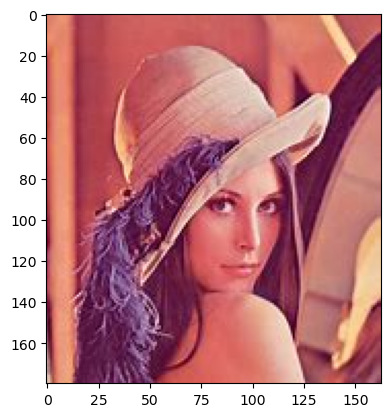
\includegraphics[width=0.22\hsize]{../img/SVD1_1000.png}}  
        \subfigure[$2$]{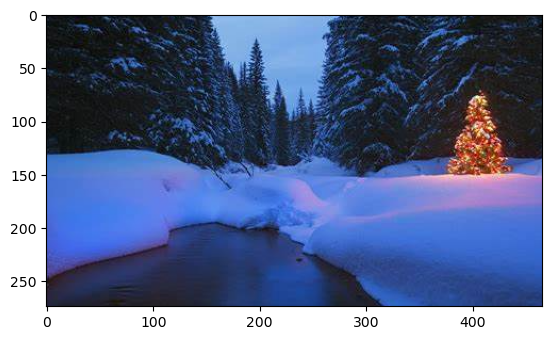
\includegraphics[width=0.22\hsize]{../img/SVD2_1000.png}} 
        \subfigure[$3$]{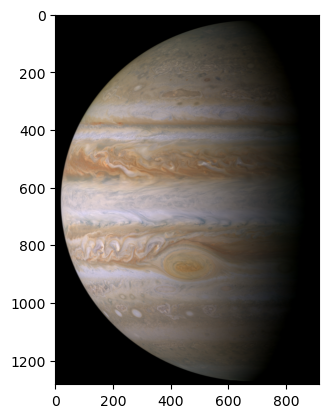
\includegraphics[width=0.22\hsize]{../img/SVD3_1000.png}}\\ %\hspace{10pt}           
        \subfigure[$SVD1_{100}$]{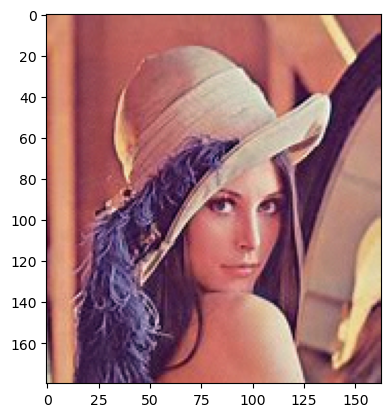
\includegraphics[width=0.22\hsize]{../img/SVD1_100.png}} 
        \subfigure[$SVD1_{50}$]{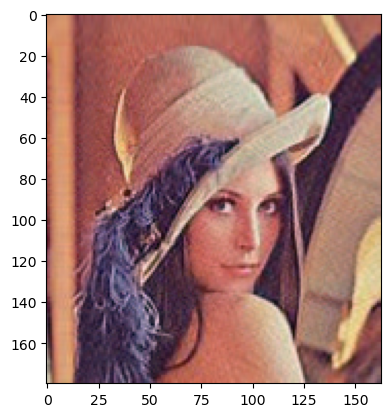
\includegraphics[width=0.22\hsize]{../img/SVD1_50.png}} 
        \subfigure[$SVD1_{30}$]{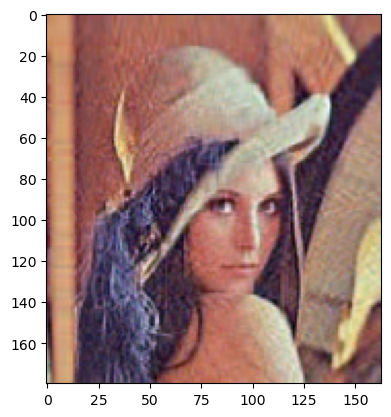
\includegraphics[width=0.22\hsize]{../img/SVD1_30.png}}\\ 
        \subfigure[$RSVD1_{100}$]{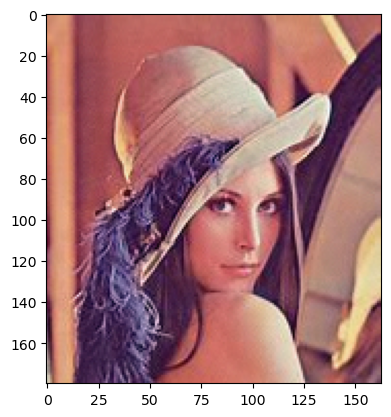
\includegraphics[width=0.22\hsize]{../img/RSVD1_100.png}}  
        \subfigure[$RSVD1_{50}$]{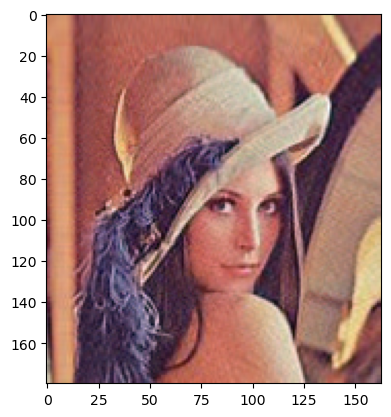
\includegraphics[width=0.22\hsize]{../img/RSVD1_50.png}} 
        \subfigure[$RSVD1_{30}$]{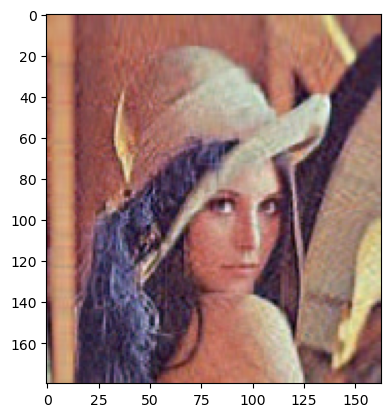
\includegraphics[width=0.22\hsize]{../img/RSVD1_30.png}}\\ %\hspace{10pt}           
        \subfigure[$SVD2_{100}$]{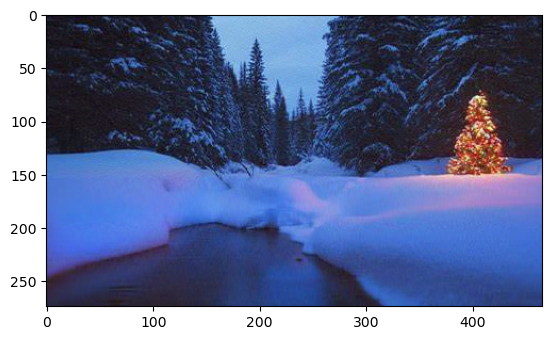
\includegraphics[width=0.22\hsize]{../img/SVD2_100.png}} 
        \subfigure[$SVD2_{50}$]{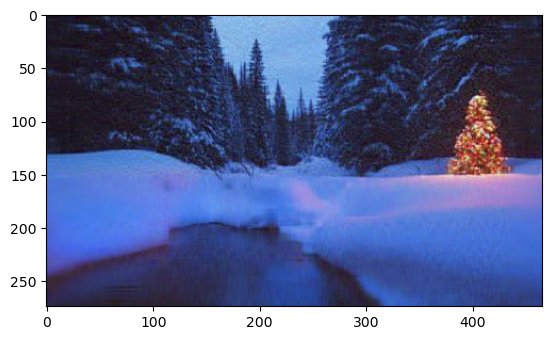
\includegraphics[width=0.22\hsize]{../img/SVD2_50.png}} 
        \subfigure[$SVD2_{30}$]{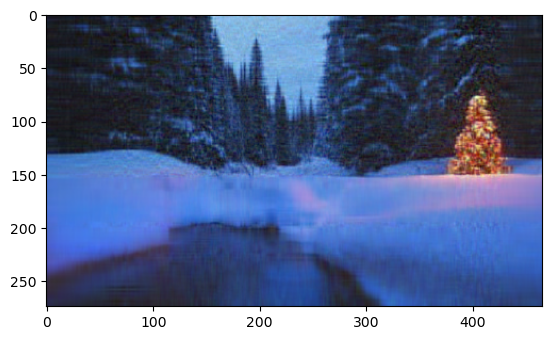
\includegraphics[width=0.22\hsize]{../img/SVD2_30.png}}\\ 
        \subfigure[$RSVD2_{100}$]{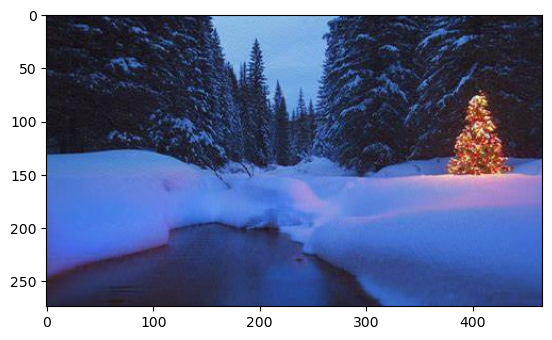
\includegraphics[width=0.22\hsize]{../img/RSVD2_100.png}}  
        \subfigure[$RSVD2_{50}$]{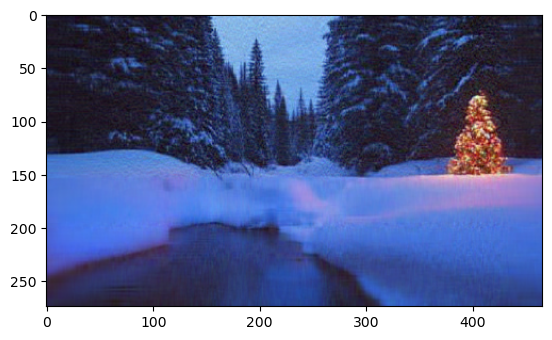
\includegraphics[width=0.22\hsize]{../img/RSVD2_50.png}} 
        \subfigure[$RSVD2_{30}$]{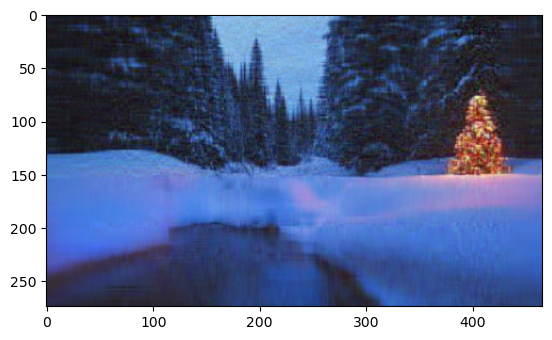
\includegraphics[width=0.22\hsize]{../img/RSVD2_30.png}}\\ %\hspace{10pt}           
        
        
\end{figure}



\begin{figure}[h!]
    \centering
    \subfigure[$SVD3_{100}$]{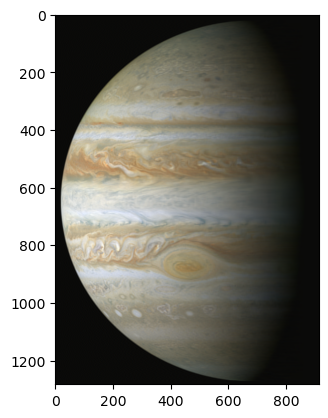
\includegraphics[width=0.22\hsize]{../img/SVD3_100.png}} 
    \subfigure[$SVD3_{50}$]{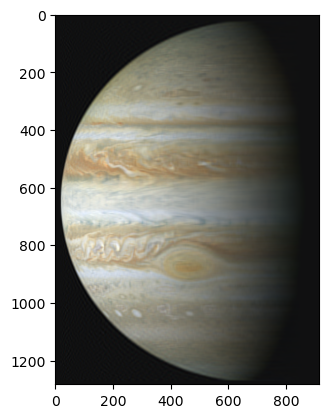
\includegraphics[width=0.22\hsize]{../img/SVD3_50.png}} 
    \subfigure[$SVD3_{30}$]{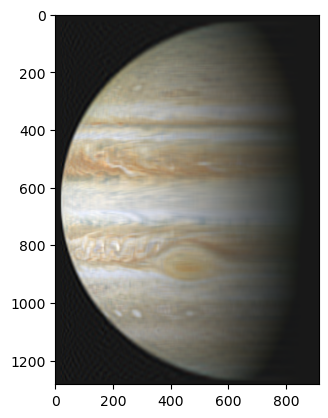
\includegraphics[width=0.22\hsize]{../img/SVD3_30.png}}\\ 
    \subfigure[$RSVD3_{100}$]{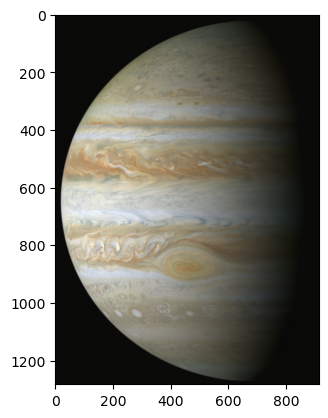
\includegraphics[width=0.22\hsize]{../img/RSVD3_100.png}}  
    \subfigure[$RSVD3_{50}$]{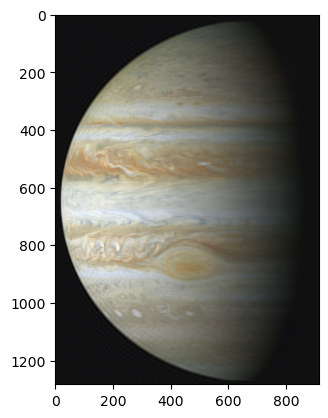
\includegraphics[width=0.22\hsize]{../img/RSVD3_50.png}} 
    \subfigure[$RSVD3_{30}$]{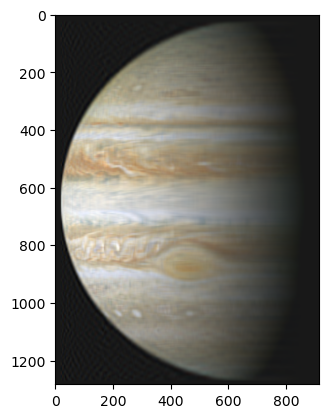
\includegraphics[width=0.22\hsize]{../img/RSVD3_30.png}}\\ 
        
    \label{wildlife}
\end{figure}




 \setcounter{section}{8}
\section*{\centerline{八、结论}}
    基于Randomized-SVD方法的图像压缩在保证图像质量相同的情况下,压缩速度较SVD方法相比快6-7倍。

 \setcounter{section}{9}
\section*{\centerline{九、问题}}
    两种算法都需要手动调整特征数参数$k$,在处理大规模数据时手动调整参数时间成本过高,设定固定参数又不能
    保证所有图像的质量。

    此外,对于整个图像来说,全局SVD可以得到全局的奇异值的对应排列,但在全局相对不重要的特征可能在图像的某个
    部分是十分重要的,因此全局SVD会造成图像局部信息丢失的问题。将图像中的数据用一个与其无关的称之为shuf的排列$S$打乱,
    然后使用SVD分解得到的矩阵$X = S(M)$,
    假设$X_r = \mathbf{U}_{r} \Sigma_{r} \mathbf{V}_{r}^{*}$表示对$X$获得的近似值。实验发现,对于相同的$r$值,图像$S^{−1} (X_r)$是一个比$M_r$更好的近似值。\upcite{ranade2007variation}




    

\bibliographystyle{plain}
\bibliography{refer}
\end{document}